\chapter{Background / Preliminaries }
\label{Preliminaries}

% In this chapter, we discuss the background information and literature related to our work. In section \ref{primitives}, we introduce two main underlying cryptography primitives in Griffin. Section \ref{2.2} presents the concept of access control, the general process of policy enforcement, and two advanced features in the distributed authorization.  Section \ref{2.3}explains several adopted contemporary web standards in the reference implementation. Section \ref{2.4} reviews the related lines of work and presents the key ideas involved in the design of our capability system. %existing literature on context confinement and permission usage control in the distributed authorization. 
% Finally, Section \ref{2.5} summarizes this chapter.


\section{TESLA}
Timed Efficient Stream Loss-tolerant Authentication(TESLA) is a light-weight protocol that provides integrity to data stream and source authentication by using digital signatures, developed by the Multicast Security (Msec) working group of the Internet Engineering Task Force (IETF). 

The main idea of TESLA is that the sender attaches to each packet a MAC computed with a key \(k\) known only to itself. The receiver buffers the received packet without being able to authenticate it. A short while later, the sender discloses \(k\) and the receiver is able to authenticate the packet. Consequently, a single MAC per packet suffices to provide broadcast authentication, provided that the receiver has synchronized its clock with the sender ahead of time.

% The basic idea of the TESLA protocol is to achieve asymmetric cryptography by delaying the disclosure of the symmetric keys. 

The whole transmission time is divided into
time intervals and packets sent in each interval have MACs using the same key, that is different key for each interval but same key for all packets in an interval. The key for interval $i$ will be disclosed to all receivers in interval $i+d$(where $d$ is delay parameter). The receiver is responsible for buffering packets until the key for their authentication has been disclosed. After disclosure the receiver can authenticate the packet, provided that the packet was received before the key was disclosed. TESLA requires loose time-synchronization between receiver and the sender as well as a bootstrap procedure to configure both receiver and sender before the data transmission.

So, we follow sequence of steps while implementing TESLA, starting with time synchronization and then adding TESLA initialization in DTLS handshake.

\textit{Limitation:TESLA is not a signature mechanism and does not provide non-repudiation, as anybody could forge authentic TESLA packets after the key is disclosed.}\\
% The asymmetry is achieved by the sender revealing an authentication key with a certain key disclosure delay after the messages authenticated with this key supposedly arrived to receivers.


% Yet this solution is limited by high computational costs and high transmission overheads.  The Timed Efficient Stream Loss-tolerant Authentication protocol (TESLA) is an alternative solution that provides the two required services, while being compatible with high rate transmissions over lossy channels.


\subsection{Building Blocks of TESLA protocol}

\begin{itemize}
\item PRNG : Pseudo-random number generator
% , e.g. ChaCha20 stream cipher, can be used.

\item PRF is the Pseudo Random Function :

\item $F$ and $F'$ : One-way hash functions. $F$ is the one-way function used to create the key chain and F' is the one-way function used to derive the HMAC keys. Implementation can use SHA-256 family algorithms.

\item Hash chain $F^{n}(K)$ denotes $n$ successive applications of cryptographic hash function $F$ to key, $K$.

\item Signature scheme 

% : $K2SN-MSS$, a post-quantum signature scheme.


\item $HMAC(K,M)$ : HMAC is the keyed-hash message authentication code which includes an underlying cryptographic hash function to create the authenticating tag.
\item \textcolor{red}{Encryption scheme \& Key-exchange scheme}.
\end{itemize}



\subsection{Assumptions}
TESLA does not need the strong time synchronization properties, but only requires loose time synchronization, and that the receiver knows an upper bound on the sender’s local time.\footnote{It is the receiver that synchronizes its time with the sender’s.}

Also, the scheme holds strong assumption that the first packet, containing synchronization details, is digitally signed by the sender, to provide authenticity to the entire stream, is not lost in transmission. TESLA is secure as long as the sender and receiver are loosely time synchronized. 


% \textcolor{red}{Additional property : Original paper \cite{perrig2000efficient} does not deal with the problem of synchronization packet lost. Here, we can achieve robustness for synchronization packet by applying some negative acknowledgement(NACK) or acknowledgement(ACK) from receiver to the sender, that is, the synchronization packet is resend after receiving NACK. We use the following notation: $S$ stands for sender, and $R$ stands for receiver. A stream $\mathcal{S}$ is divided into chunks $<M_{1}, M_{2} \cdots M_{n}>$. }

\subsection{Time Synchronization}  
\label{TimeSyncronization}
The security offered by TESLA work according to a strict time schedule. Therefore the session's sender and each receiver need to have synchronized clocks. Fig \ref{timeSync} shows a basic time synchronization by Perrig  et al. in \cite{perrig2002tesla}.

\begin{figure}[H]
    \centering
    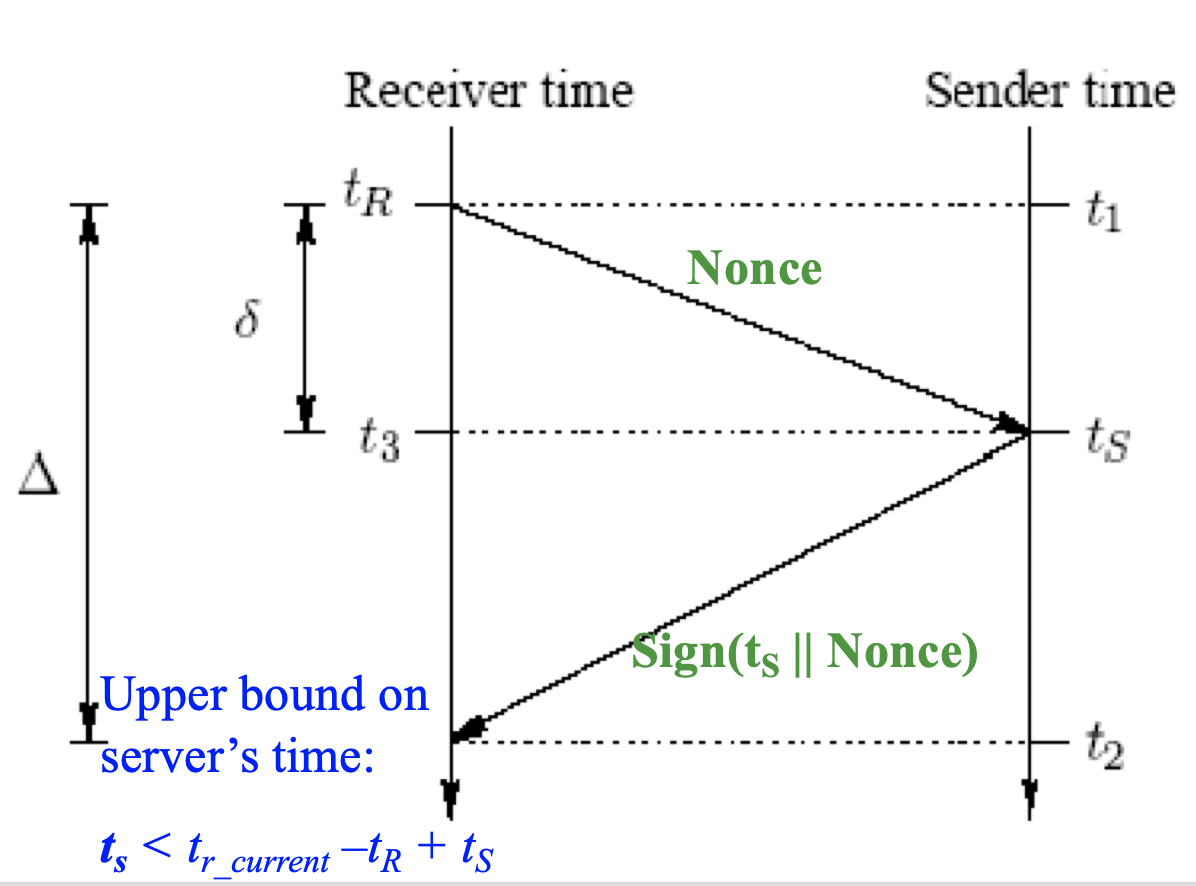
\includegraphics[height=7cm,width=8cm]{figures/timeSync.png}
    \caption{Synchronization Scheme : Calculation of upper bound on server’s time}
    \label{timeSync}
\end{figure}

We know that : $t_{s} = t_{Rcurr} + t_{S} - t_{R}$ from time synchronization given in \cite{perrig2002tesla} and shown in fig \ref{timeSync}.


This $ \delta= t_{S} - t_{R}$ is the real time synchronization. The receiver should keep this value to calculate upper bound on sender's clock. 



\subsection{TESLA Algorithm 4 Description:}
In previous TESLA schemes defined in \cite{perrig2000efficient}, a fixed or predictable sender schedule is used, with each recipient knowing the exact sending time of each packet. Since this severely restricts the flexibility of senders, we use the scheme 4 which allows senders to send at dynamic transmission rates, without the requirement that every receiver needs to know about the exact sending schedule of each packet. 

The solution to this problem is to pick the MAC key and the disclosed key in each packet only on a time interval basis instead of on a packet index basis. The sender uses the same key $K_{i}$ compute the MAC for all packets which are sent in the same interval $i$. All packets sent in interval $i$ disclose the key $K_{i-d}$, where $d$ is disclosure delay.\\

 We use algorithm 4 of TESLA\cite{perrig2000efficient} as shown in figure \ref{teslaAlgo4}.\\
 
\textbf{Initial Synchronization}(Refer Fig. \ref{InitialSynchronization})
\begin{enumerate}
\item The receiver sends a request(nonce) that it wants to receive packets from the sender.
\[Receiver \xrightarrow{\text{nonce}}Sender\]
\item When the sender gets a request from a receiver, the sender first generates a secret key(or commitment key), using any PRNG. This key is used to generate a key chain.

\item The sender is the one generating the key chain, using a one-way hash function for both key chain and dervivation of hmac keys, as shown in figure \ref{tesla(keygen)} :
    
    \begin{figure}[H]
    \centering
    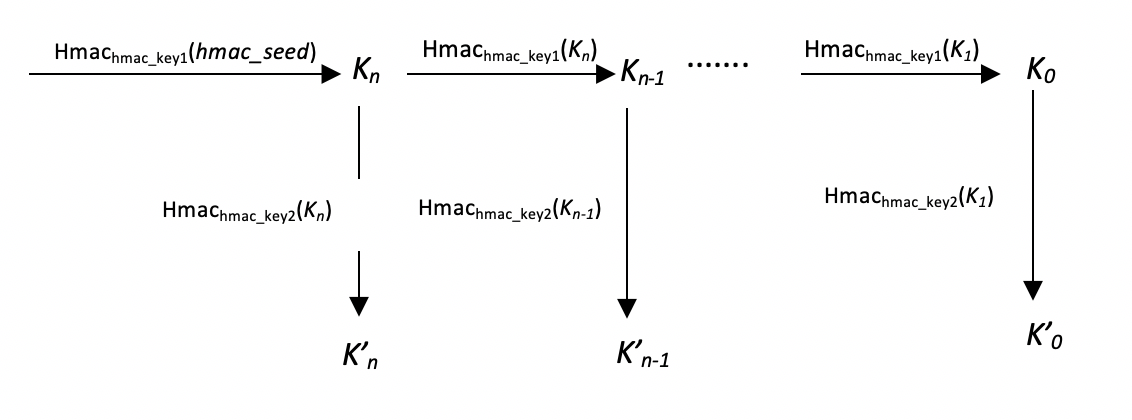
\includegraphics[height=4cm,width=10cm]{figures/tesla(keygen).png}
    \caption{Key Chain in TESLA :  The keys $K_{i}$ are derived from $hmac_{key1}$ and $hmac_{seed}$, while the hmac keys $K'_{i}$ are derived from another hmac called $hmac_{key2}$ and $K_{i}$}
    \label{tesla(keygen)}
    \end{figure}

\item Sender prepares a synchronization response packet, signed by sender's private key, that uses $K2SN-OTS$. We use K2SN-OTS for signing each such Synchronization Packet.

The synchronization response packet is defined as, \[SynRes= \{{T_{s},Nonce,r,i,T_{start}, K_{j},d,n}\}_{K2SN\-OTS_{i}}\], parameters defined in table \ref{notationTable}.


\end{enumerate}
\begin{figure}[H]
    \centering
    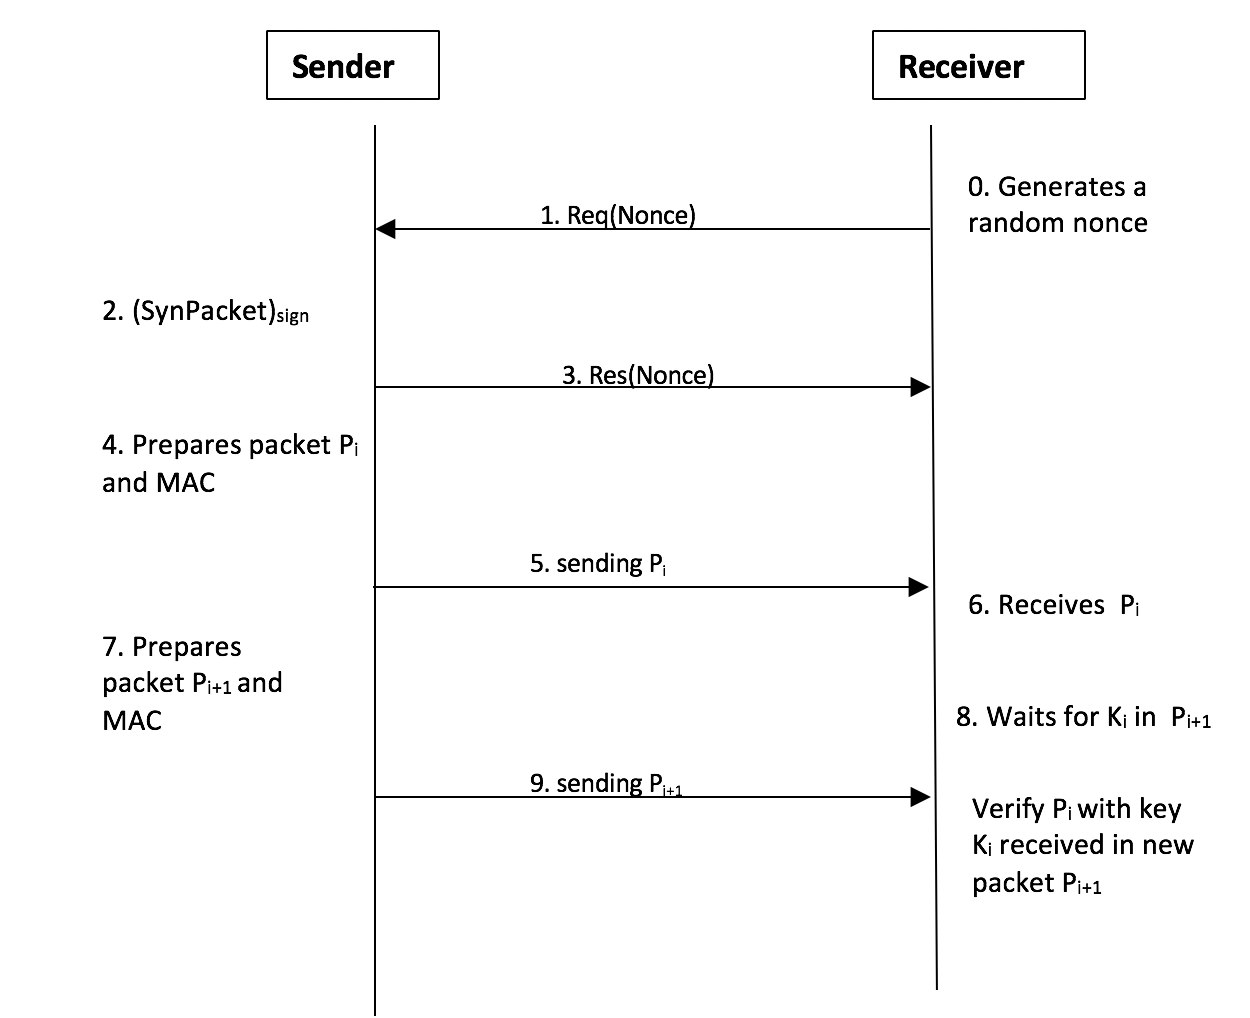
\includegraphics[height=7cm,width=8.5cm]{figures/tesla1.png}
    \caption{Initial Synchronization : Sender sends data packets to Receiver}
    \label{InitialSynchronization}
\end{figure}

\textbf{Broadcasting Authenticated Messages}
The sender broadcasts the messages after initial synchronization is complete.
To broadcast message $M_{j}$ in interval $i$ the sender constructs packet \[P_{j} = \{M_{j} \|i\|  K_{i-d}\|MAC(K'_{i} , M_{j} ) \}\].




% \begin{figure*}[!ht]
% \centering
% 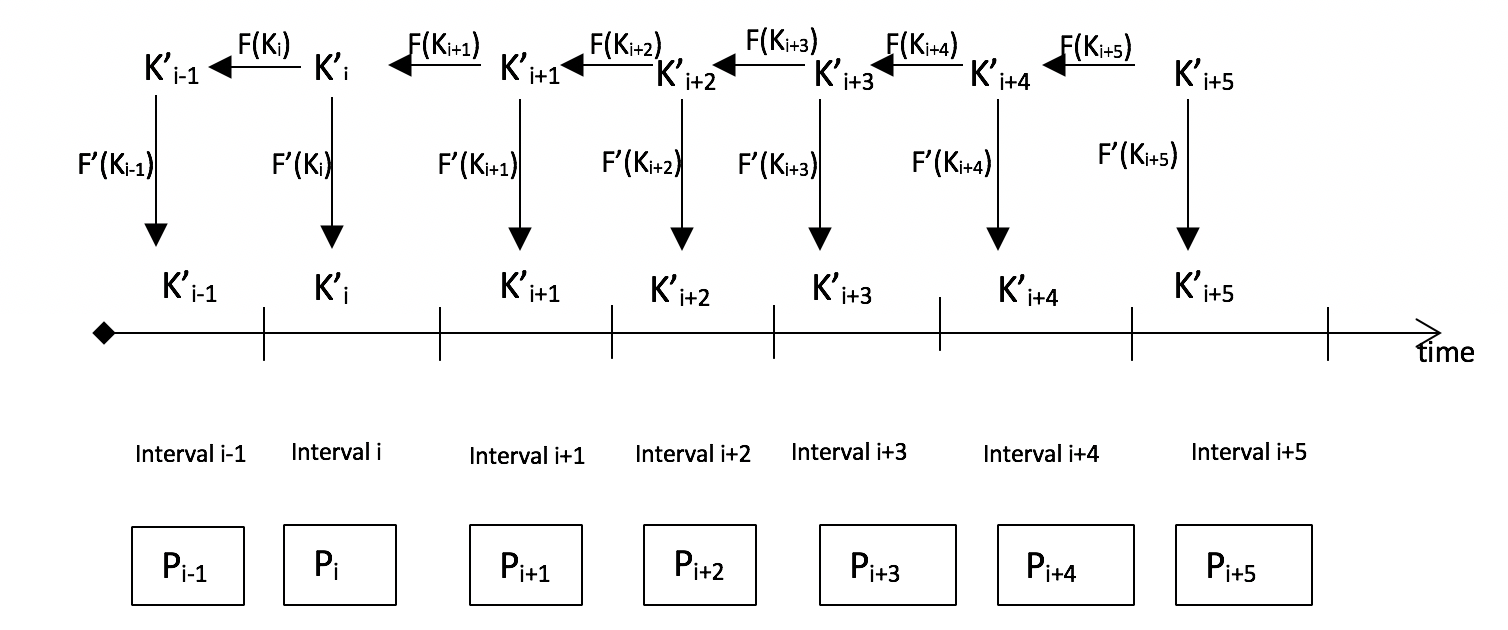
\includegraphics[width=0.9\textwidth]{figures/teslaAlgo3.png}
% \caption{TESLA Algorithm 3 : At the top of the figure is the one-way key chain (using the one-way function F), and the derived MAC keys (using the one-way function F'). Time advances left-to-right, is split into time intervals of uniform duration. At the bottom of the figure, sender sends packet in each time interval and uses the corresponding key to that time interval to compute the MAC of the packet. 
% Ex: Key used for packet $P_{i}$ in interval $i$, is revealed in packet $P_{i+2}$, which arrives in interval $i+2$, assuming a key disclosure delay of two time intervals (d = 2).}
% \label{teslaAlgo3}
% \end{figure*}

% \begin{table*}[!ht]
% 
\begin{figure*}[H]
\centering
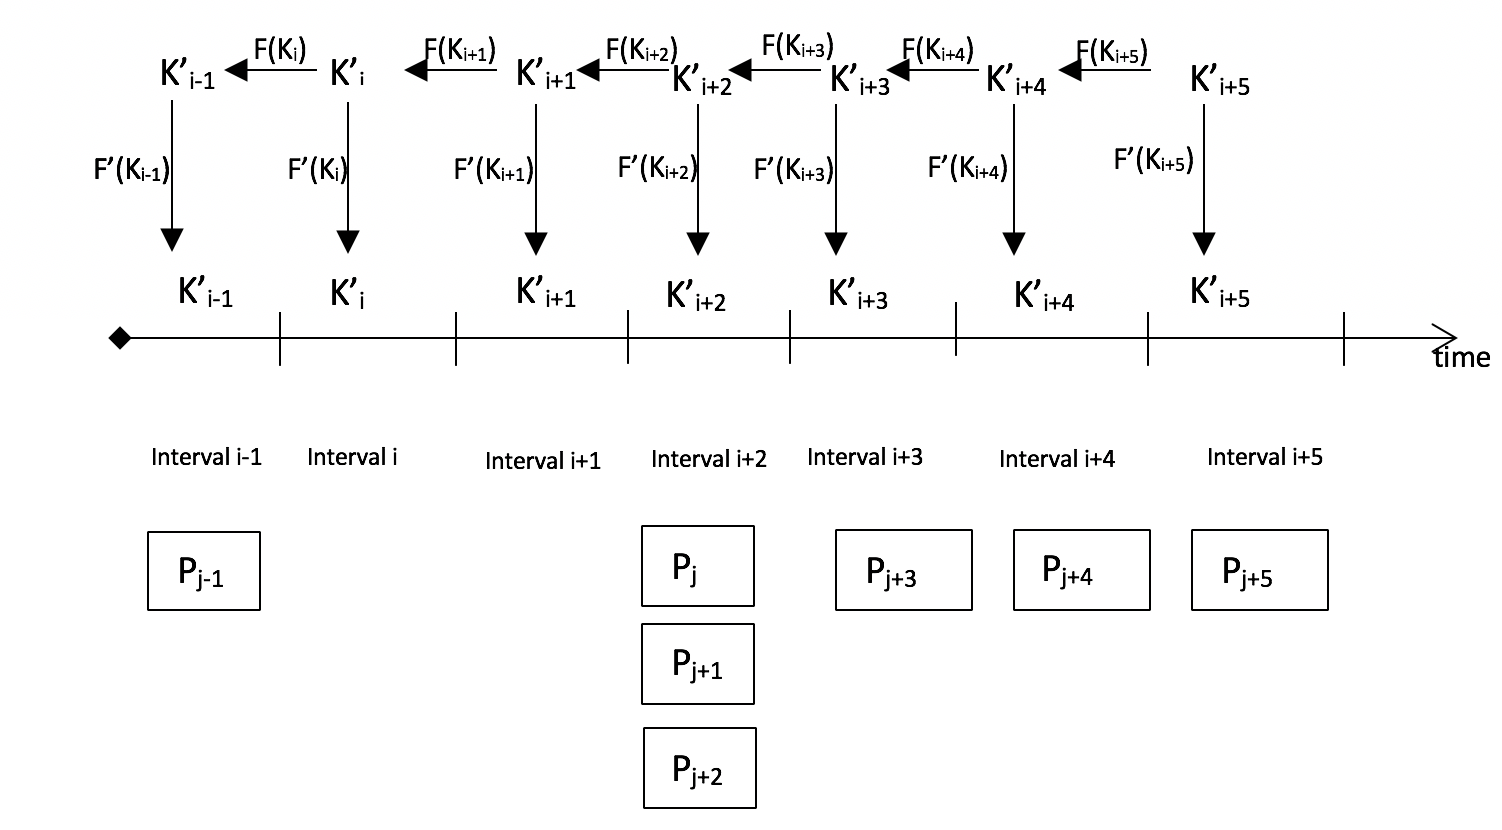
\includegraphics[width=0.8\textwidth]{figures/teslaAlgo4.png}
\caption{TESLA Algorithm 4 :At the top of the figure is the one-way key chain (using the one-way function F), and the derived MAC keys (using the one-way function F'). Time advances left-to-right, is split into time intervals of uniform duration. At the bottom of the figure, sender sends packet in each time interval and uses the corresponding key to that time interval to compute the MAC of the packet. Here, we do not limit packets per interval, so the rate of transmission by sender can vary. 
Ex: Key used for all packets in interval $i+2$ is same, and is revealed in packet $P_{j+4}$, which arrives in interval $i+4$, assuming a key disclosure delay of two time intervals (d = 2).}
\label{teslaAlgo4}
\end{figure*}


\textbf{Authentication at Receiver}
A receiver must first receive a packet containing the bootstrap information, digitally signed by the sender, and verify its signature. Two actions must be performed by receiver before the authentication of actual data packets :

$\bullet$ Receive and process a bootstrap information message, and

$\bullet$ Calculate an upper bound of the sender's local time. To that purpose, the receiver must perform time synchronization.

After initial synchronization, when a sender discloses a key, all parties potentially have access to that key commitment. So as packets arrive, the receiver
must verify that their MACs are based on security condition\footnote{Security condition: A data packet $P_{i}$ arrived safely, if the receiver can unambiguously decide, based on its synchronized time and $\delta_{t}$ that the sender did not yet send out the corresponding key disclosure packet $P_{j}$}.\\

% \begin{algorithm}[h]
% \DontPrintSemicolon
% \SetAlgoLined
% \SetNoFillComment
% \LinesNotNumbered 
% %\SetSideCommentLeft
% \tcc{iterate over all training examples}
%  \KwData{this text}
%  \KwResult{how to write algorithm with \LaTeX2e }
%  initialization\;
%  \While{not at end of this document}{
%   read current \tcp*[l]{will be used to compute $\partial x$}
%   \eIf{understand}{
%   go to next section \tcp*{will be used to compute $\partial x$}
%   current section becomes this one\;
%   }{
%   go back to the beginning of current section\;
%   }
%  }
%  \caption{How to write algorithms}
% \end{algorithm}

% \usepackage{xcolor}
% \usepackage{algorithm}
% \usepackage[noend]{algpseudocode}



	
\begin{algorithm}[H] %[!ht]
\caption{RECEIVER : Authentication of Received Packets}
\begin{algorithmic}[1]
\State \texttt{Input : $P_{j}$ }
\State \texttt{Output : True/False\footnote{(True will accept the packet, while False will reject the packet)} }
\State
\Procedure{AuthDataPacket}{$P_{j}$}
\State Safe Packet check for packet $P_{j}$ 
\State T =  Arrival time of $P_{j}$
\State \texttt{$t_{j}=T+D_{t}$}
\State \texttt{$T_{sender_{i}}= \frac{ t_{j} - T_{0} } { T_{int} }  $}

\If{$T_{sender_{i}} < (i+d)$}
    \State\texttt{\textbf{print} "Packet $P_{j}$ is SAFE"}
    \State Key Verification
    % \State
    % \State
    % \tcp{(1) Extract legitimate key from the key chain}
    \State \texttt{Extract $K_{v}$}
    \State \texttt{$K'_{v}=F'^{(i-d-v)}(K_{i-d})$ }
        \If {($v < (i-d)) \&\& (K'_{v}==K_{v}$)}
            \State \texttt{\textbf{print} "Key is VERIFIED"}
            \State HMAC Verification
            \For{\texttt{each $h \in w$, where, $w= \{(v+1) \cdots (i-d-1)\}$ time-intervals}}
            \State To authenticate a buffered packet $P_{h}$ 
                \State \texttt{$K'_{h}=F(K_{h})$}
                \State $hmac=$\texttt{Extract HMAC of $P_{h}$}
                \State $hmac' =HMAC(K'_{h},M_{h}))$
                \If{ $hmac=hmac'$}
                  \texttt{Packet $P_{h}$ is AUTHENTICATED}
                    % \State \texttt{exit;}
                \Else
                    \texttt{continue to next packet}
                \EndIf
            \EndFor all packets buffered
        \Else 
            \State \texttt{\textbf{print} "Key is UN-VERIFIED"}
             \State \textbf\texttt{{break;}}
        \EndIf
\Else 
        \State \textbf{\texttt{print}} \texttt{"Packet $P_{j}$ is UN-SAFE"}
        \State \textbf{return} \textcolor{red}{FALSE};
    \EndIf
\State \textbf{return} \textcolor{green}{TRUE};
\EndProcedure
\label{ReceiverTeslaAlgo}
\end{algorithmic}
\end{algorithm}




Step-wise TESLA authentication, when a sender sends packet $P_{j}$ in interval $i$, is explained below:
\begin{enumerate}
    \item When the receiver receives packet $P_{j}$ , the receiver can use the self-authenticating key $K_{i-d}$ disclosed in $P_{j}$ to determine $i$.
    \item Receiver checks the latest possible time interval $x$ the sender could currently be in (based on the loosely synchronized clock). If $x<(i+d)$ (recall that $d$ is number of intervals that the key disclosure is delayed) then the packet is safe.
    \item The sender has thus not yet reached the interval where it discloses $K_{i}$, the key that will verify packet $P_{j}$.
    \item The receiver cannot yet verify the authenticity of packet  $P_{j}$ sent in interval $i$, so, it adds the triplet $\{i, M_{j} , MAC(K'_{i}, M_{j} )\}$ to a buffer, and verifies the authenticity after it learns $K'_{i}$.
\end{enumerate}


 
     
% \begin{figure}[H]
%     \centering
%     \includegraphics[height=1cm,width=16cm]{figures/teslahand.png}
%     \caption{TESLA Initialization Overhead}
%     \label{teslahead}
% \end{figure}

% \begin{figure}[H]
%     \centering
%     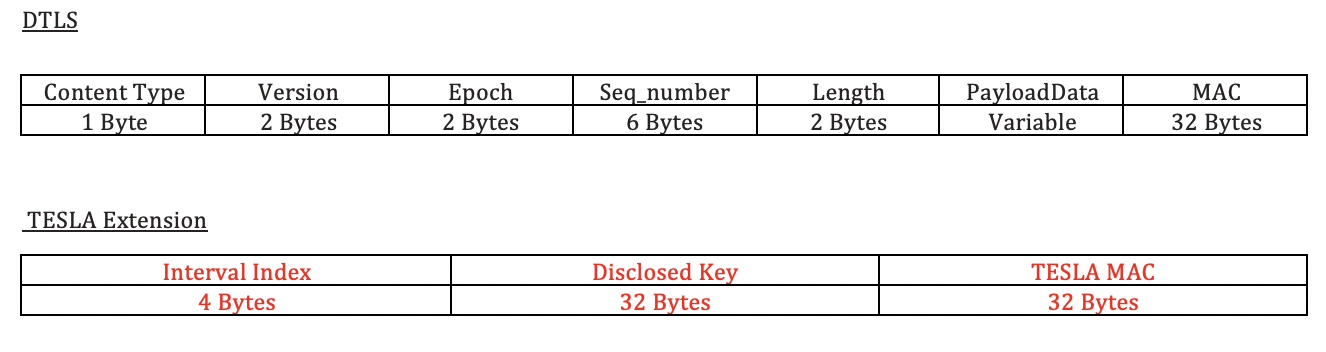
\includegraphics[height=5cm,width=16cm]{figures/packetOverhead.png}
%     \caption{TESLA Per Data packet Overhead}
%     \label{packetOverhead}
% \end{figure}













%%%%%%%%%%%%%%%%%%%%%%%%%%%%%%%%%%%%%%%%%%%%%%%%%%%%%%%%%%%
\section{DTLS}
\label{dtls}
Datagram Transport Layer Security is a network communication security protocol that enables two parties to establish a secure session and protect data exchange over the corresponding connection(Fig. \ref{workMechanism(dtls)}). As a security protocol DTLS aims to achieve the four security objectives- confidentiality, message integrity, peer authentication and non-repudiation  over UDP channel.\cite{kothmayr2013dtls}. 
The DTLS protocol is designed to secure data between communicating applications.  It is designed to run in application space, without requiring any kernel modifications. 
DTLS provides data stream authentication for applications built on User Datagram Protocol(UDP) channel, by using explicit sequence numbers in the data packets to provide stream authentication. To provide authenticity, it uses HMAC in each packet. The key to calculate HMAC for each packet is same and is established during handshake.

%height=5cm,width=8cm [!ht]
\begin{figure}[H]
\centering
    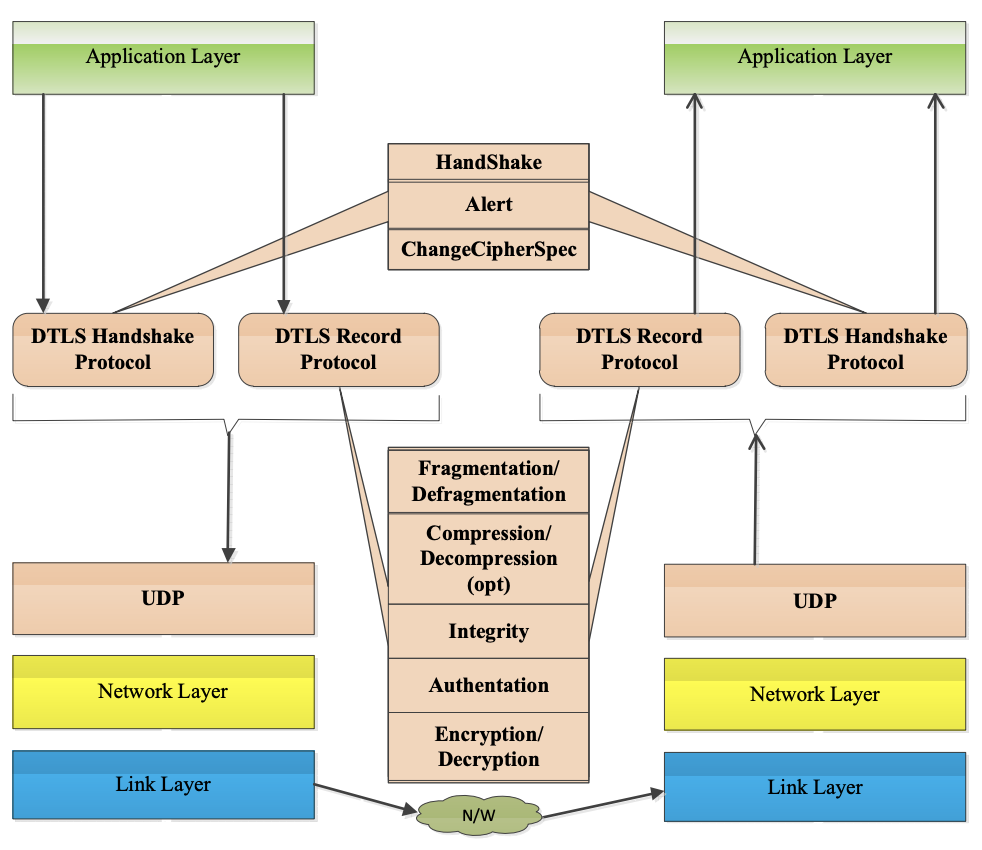
\includegraphics[height=6cm,width=8.5cm]{figures/workMechanism(dtls).png}
    \caption{OSI Model of DTLS Application}
    \label{workMechanism(dtls)}
\end{figure}



\subsection{Security Guarantees}
DTLS provides three key services:
\begin{enumerate}
    \item Confidentiality: Ensuring that anyone intercepting the communications between the client and server cannot decipher that content. 
    
    The confidentiality is ensured by leveraging symmetric cryptography, the keys of which are negotiated during a TLS handshake.
    
    \item Authentication: Ensuring that a client is in fact talking to the server that the client thinks it is talking to. Optionally, the server can authenticate the client, but this is rare.
    
    The authenticity is established by using certificates, once again exchanged during the initial handshake, and maintained through the session using either \textsf{HMAC} (Hashed Message Authentication Codes) or AEAD (Authenticated Encryption with Associated Data), depending on the negotiated cipher suite.
    
    \item Integrity: Ensuring that the messages and communication have not been corrupted or tampered with.
  
  The integrity is ensured by using a Message Authentication Code (MAC).
\end{enumerate}

A DTLS connection contains two main phases: DTLS Handshake Protocol and Record Layer Protocol.



\subsection{DTLS Handshake Protocol}
The Handshake is responsible for negotiating session keys and cryptographic algorithms, and key agreement is either based on public key cryptography (the standard case), or on pre-shared keys. The set of algorithms to be used is specified in a cipher suite. It performs key exchange, source authentication, encryption and hash algorithms to be used in record protocol. \textit{Secure session is established after Finish message which checks integrity of previous HS messages using keys and cryptographic algorithms agreed during the handshake.}The TLS handshake is authenticated using the Finished messages as usual.
The DTLS handshake in fig. \ref{dtls(auth)} has three phases  : 
\begin{enumerate}
        \item Key Exchange: Establish shared keying material and select the cryptographic parameters.the client and server, both need to generate matching keys for use with the selected algorithms.  Everything after \textit{ServerHello} phase is encrypted.
        \item Server Parameters: Establish other handshake parameters (whether the client is authenticated, application layer protocol support, etc.).
        \item Authentication: Authenticate the server (and optionally the client) and provide key confirmation and handshake integrity.
\end{enumerate}
Like TLS, DTLS also has a base protocol called Record Layer,  and four sub-protocols on top,namely Handshake,  ChangeCipherSpec,  Alert Protocol and the application data protocol as shown in figure \ref{workMechanism(dtls)}. The diaram shows the OSI layer and how two end points communicates with DTLS as the security layer.
\begin{figure}[H]
\centering
    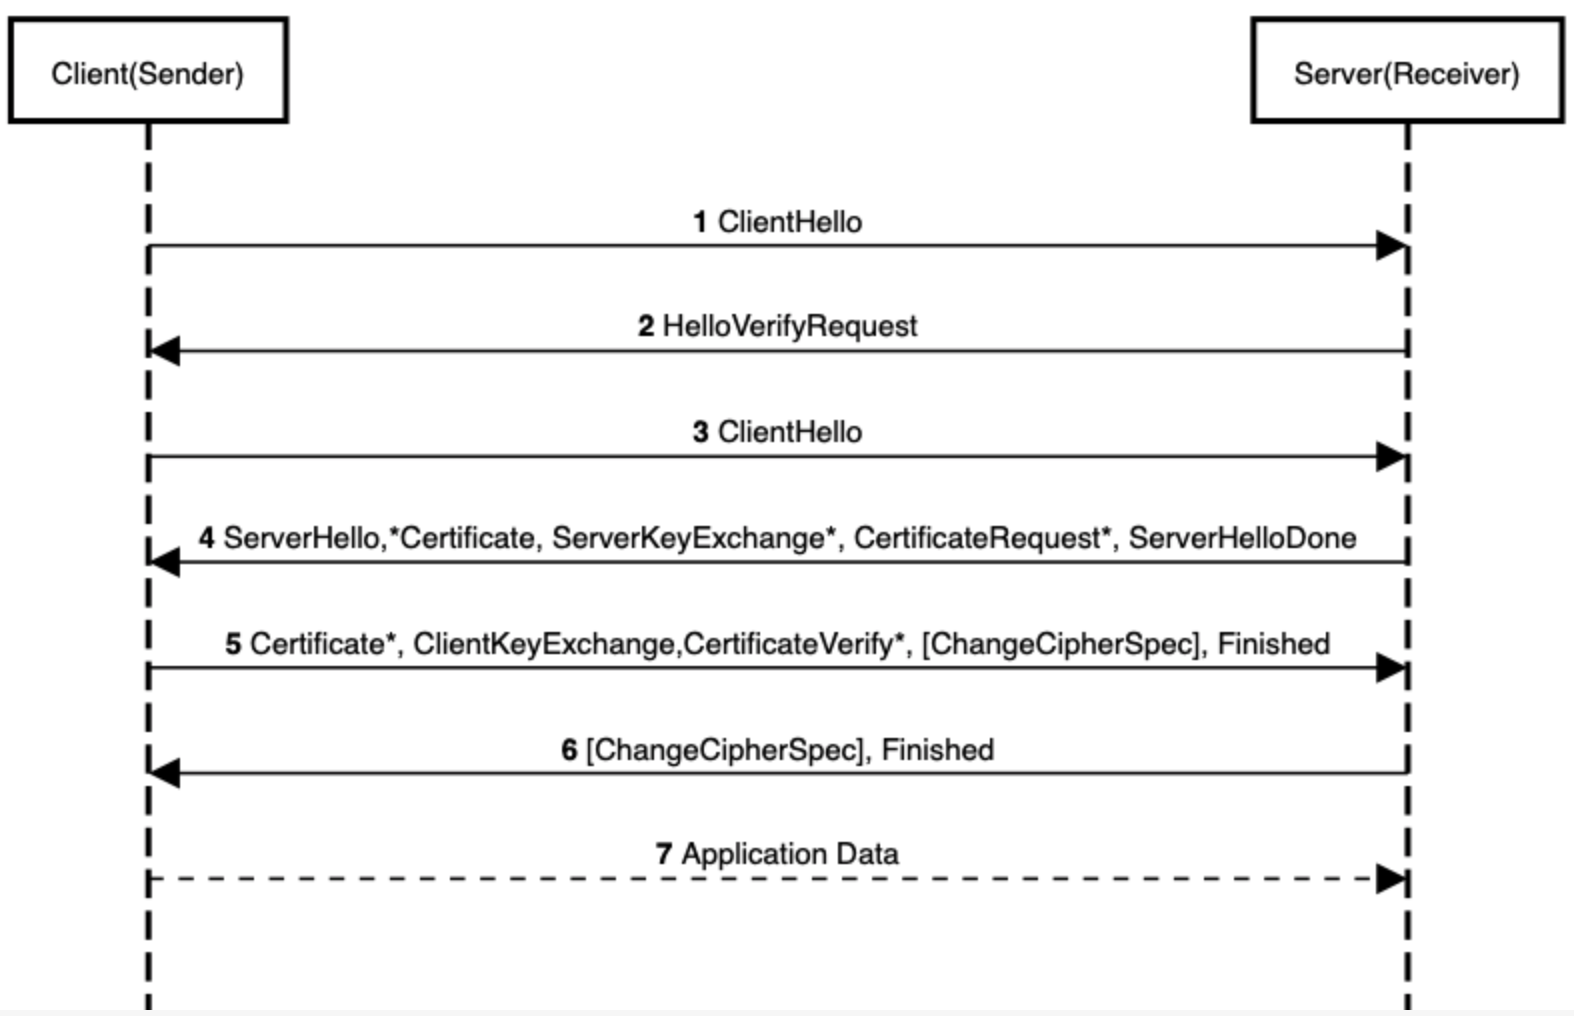
\includegraphics[height=10cm,width=12cm]{figures/dtls(auth).png}
    \caption{DTLS Fully Authenticated Handshake}
    \label{dtls(auth)}
\end{figure}

\begin{enumerate}
\item The DTLS \textit{ClientHello} message contains a cookie field. The initial \textit{ClientHello} contains an empty (zero-length) cookie or potentially one cached from a prior exchange.

\item A server that is unable to verify the incoming cookie and wishes to establish the liveness of the DTLS client sends a \textit{HelloVerifyRequest} message. (Note : Servers that are more sensitive to overall handshake latency can skip the \textit{HelloVerifyRequest} message and instead respond with \textit{ServerHello} messages, in which case the protocol flow is the same as in TLS.)

\par The \textit{HelloVerifyRequest} message contains a cookie. This cookie should be generated in such a way that it does not require keeping state on the server, thus avoiding memory consumption denial of service attacks. For example, the cookie can be generated from a keyed hash of the client IP address, using a global key.

\item Unlike application data, handshake messages(including the \textit{ChangeCipherSpec} message) must be reliably delivered since all handshake messages are necessary for successful session negotiation. This creates three problems: 
\begin{enumerate}
\item First, messages may be lost on the network.Once the client has transmitted the \textit{ClientHello} message, it expects to see a \textit{HelloRetryRequest} from the server. However, if the server’s message is lost, the client knows that either the \textit{ClientHello} or the \textit{HelloRetryRequest} has been lost and retransmits. When the server receives the retransmission, it knows to retransmit. The server also maintains a retransmission timer and retransmits when that timer expires.
	
\item	Second, they may be reordered, confusing the receiving peer.In DTLS, each handshake message is assigned a specific sequence number within that handshake. When a peer receives a handshake message, it can quickly determine whether that message is the next message it expects. If it is, then it processes it. If not, it queues it for future handling once all previous messages have been received.

\item	Third, some handshake messages are too large to fit in a single DTLS record and therefore must be fragmented across multiple records. TLS and DTLS handshake messages can be quite large (in theory up to \(2^{24}-1\) bytes, in practice many kilobytes). By contrast, UDP datagrams are often limited to less than 1500 bytes if IP fragmentation is not desired. In order to compensate for this 	limitation, each DTLS handshake message may be fragmented over several DTLS records, each of which is intended to fit in a single IP datagram. Each DTLS handshake message contains both a fragment offset and a fragment length. Thus, a recipient in possession of all bytes of a handshake message can reassemble the original unfragmented message.

\end{enumerate}
    \item All handshake messages after the ServerHello are now encrypted. The newly introduced EncryptedExtension message allows various extensions previously sent in clear in the ServerHello to also enjoy confidentiality protection.
    \item The purpose of Finished messages is to verify that parties have correctly negotiated keys and algorithms.
\end{enumerate}
   
   
\subsubsection{Use of PSK}
There are three types of ciphersuits that use PSK \href{https://tools.ietf.org/html/rfc4279#section-5.1}{RFC4279}

\begin{enumerate}
    \item PSK : Use only symmetric key algorithms and are thus especially suitable for performance-constrained environments. 
    \item DHE\_PSK ciphersuites : Use a PSK to authenticate a Diffie-Hellman exchange.  These ciphersuites protect against dictionary attacks by passive eavesdroppers (but not active attackers) and also provide Perfect Forward Secrecy (PFS).
    \item RSA\_PSK ciphersuites : combine public-key-based authentication of the server (using RSA and certificates) with mutual authentication using a PSK.
\end{enumerate}

As with all schemes involving shared keys, special care should be taken to protect the shared values and to limit their exposure over time.


\begin{enumerate}
    \item Perfect Forward Secrecy (PFS) : The PSK and RSA\_PSK ciphersuites defined in this document do not provide Perfect Forward Secrecy (PFS).  That is, if the shared secret key (in PSK ciphersuites), or both the shared secret key and the RSA private key (in RSA\_PSK ciphersuites), is somehow compromised, an attacker can decrypt old conversations. The DHE\_PSK ciphersuites provide Perfect Forward Secrecy if a fresh Diffie-Hellman private key is generated for each handshake.

    \item Brute-Force and Dictionary Attacks : Use of a fixed shared secret of limited entropy (for example, a PSK that is relatively short, or was chosen by a human and thus may contain less entropy than its length would imply) may allow an attacker to perform a brute-force or dictionary attack to recover the secret.  This may be either an off-line attack (against a captured. TLS handshake messages) or an on-line attack where the attacker attempts to connect to the server and tries different keys.

    For the PSK ciphersuites, an attacker can get the information required for an off-line attack by eavesdropping on a TLS handshake, or by getting a valid client to attempt connection with the attacker. \footnote{This one is used in our implementation in TinyDTLS.}
    
    \item Identity Privacy : The PSK identity is sent in cleartext.  Although using a user name or other similar string as the PSK identity is the most straightforward option, it may lead to problems in some environments since an eavesdropper is able to identify the communicating parties.  Even when the identity does not reveal any information itself, reusing the same identity over time may eventually allow an attacker to perform traffic analysis to identify the parties.  

\end{enumerate}

\textit{Alternative to PSK : If the main goal is to avoid Public-Key Infrastructures (PKIs), another possibility worth considering is using self-signed certificates with public key fingerprints.  Instead of manually configuring a shared secret in, for instance, some configuration file, a fingerprint (hash) of the other party's public key (or certificate) could be placed there instead.}


\subsubsection{Integrity check in handshake messages}
A Finished message is always sent immediately after a change cipher spec message to verify that the key exchange and authentication processes were successful.  It is essential that a change cipher spec message be received between the other handshake messages and the Finished message.

The Finished message is the first one protected with the just negotiated algorithms, keys, and secrets.  Recipients of Finished messages MUST verify that the contents are correct.  Once a side has sent its Finished message and received and validated the Finished message from its peer, it may begin to send and receive application data over the connection.


Structure of this message:
\label{struct1}
\begin{lstlisting}
struct {
          opaque verify_data[verify_data_length];
      } Finished;

\end{lstlisting}      
     
\begin{lstlisting}
verify_data
        PRF(master_secret, finished_label, Hash(handshake_messages)) 
        [0..verify_data_length-1];

\end{lstlisting}    
      

\vspace{1cm}$finished\_label$
         For Finished messages sent by the client, the string
         "client finished".  For Finished messages sent by the server,
         the string "server finished".

$Hash$ denotes a Hash of the handshake messages.
$handshake\_messages$: All of the data from all messages in this handshake (not including any $HelloRequest$ messages) up to, but not including, this message.  This is only data visible at the handshake layer and does not include record layer headers.  This is the concatenation of all the Handshake structures as defined in Section 7.4, exchanged thus far.


The value $handshake\_messages$ includes all handshake messages starting at $ClientHello$ up to, but not including, this Finished message.  Also, the $handshake\_messages$ for the Finished message sent by the client will be different from that for the Finished message sent by the server, because the one that is sent second will include the prior one.

\subsection{Record Protocol}
The Record Layer splits the received cleartext data stream into DTLS Records. Handshake messages are also sent as records (typically unencrypted), and after the ChangeCipherSpec message is sent in the handshake, the content of all subsequent records is encrypted using the negotiated session keys—where different keys are used for the two communication directions.



\subsection{Fragmentation Issues} \cite{rfc6347}
In general, DTLS's philosophy is to leave PMTU discovery to the
   application.  However, DTLS cannot completely ignore PMTU for three
   reasons:
\begin{enumerate}
    \item The DTLS record framing expands the datagram size, thus lowering
      the effective PMTU from the application's perspective.

   \item  In some implementations, the application may not directly talk to
      the network, in which case the DTLS stack may absorb ICMP
      [RFC1191] "Datagram Too Big" indications or ICMPv6 [RFC4443]
      "Packet Too Big" indications.

   \item The DTLS handshake messages can exceed the PMTU.
\end{enumerate}{}
 In order to deal with the first two issues, the DTLS record layer
   SHOULD behave as described below.


   If PMTU estimates are available from the underlying transport
   protocol, they should be made available to upper layer protocols.  In
   particular:
\begin{enumerate}
    \item For DTLS over UDP, the upper layer protocol SHOULD be allowed to obtain the PMTU estimate maintained in the IP layer.
      
    \item  For DTLS over DCCP, the upper layer protocol SHOULD be allowed to obtain the current estimate of the PMTU.

   \item For DTLS over TCP or SCTP, which automatically fragment and
      reassemble datagrams, there is no PMTU limitation.  However, the
      upper layer protocol MUST NOT write any record that exceeds the
      maximum record size of $2^{14}$ Bytes.
      
\end{enumerate}{}


The DTLS record layer SHOULD allow the upper layer protocol to discover the amount of record expansion expected by the DTLS processing.  Note that this number is only an estimate because of block padding and the potential use of DTLS compression.

If there is a transport protocol indication (either via ICMP or via a refusal to send the datagram as in Section 14 of [DCCP]), then the DTLS record layer MUST inform the upper layer protocol of the error.

The DTLS record layer SHOULD NOT interfere with upper layer protocols performing PMTU discovery, whether via [RFC1191] or [RFC4821] mechanisms.  In particular:\\
\begin{enumerate}
    \item Where allowed by the underlying transport protocol, the upper
      layer protocol SHOULD be allowed to set the state of the DF bit
      (in IPv4) or prohibit local fragmentation (in IPv6).
     \item If the underlying transport protocol allows the application to request PMTU probing (e.g., DCCP), the DTLS record layer should honor this request.
\end{enumerate}{}


The final issue is the DTLS handshake protocol.  From the perspective of the DTLS record layer, this is merely another upper layer protocol.  However, DTLS handshakes occur infrequently and involve only a few round trips; therefore, the handshake protocol PMTU
handling places a premium on rapid completion over accurate PMTU discovery.  In order to allow connections under these circumstances, DTLS implementations SHOULD follow the following rules:
\begin{enumerate}
    \item If the DTLS record layer informs the DTLS handshake layer that a message is too big, it SHOULD immediately attempt to fragment it, using any existing information about the PMTU.
    \item If repeated retransmissions do not result in a response, and the PMTU is unknown, subsequent retransmissions SHOULD back off to a smaller record size, fragmenting the handshake message as appropriate.  This standard does not specify an exact number of retransmits to attempt before backing off, but 2-3 seems appropriate.
\end{enumerate}{}

Since Handshake messages will be larger than 1500Bytes, we need to make sure that DTLS supports fragmentation, for future.

DTLS offers fragmentation at the handshake layer, however this can add a significant overhead due to packet loss and the need for a buffer to enable message re-ordering.


The handshake header contains the overall message length, a message sequence number (MSN, message seq), as well as the fragment offset (frag offset) and its length (frag length). These information ensure that handshake fragments can be ordered and reassembled correctly. As previously stated, DTLS does not support fragmentation for the record layer. Fragmentation is only supported for handshake messages.


As part of the handshake process, the server sends its list of trusted root certificates to the client in the form of a non-encrypted record. This is done so that if the server requires that the client have a digital certificate for authentication, the client is able to select one that will chain up to a root certificate trusted by the server. While there is no defined limit on the number root certificates that can be in this list, there is a limitation on the size of the records exchanged between the client and the server. This limit is defined in RFC 2246 as 16,384 bytes.
So how does the Handshake protocol handle those scenarios where the list of trusted root certificates exceeds 16,384 bytes? RFC 2246 describes a process called record fragmentation, where any data that would exceed the 16KB record limit is split across multiple fragments. These fragments must be merged into one record by the client in order to retrieve the data. \cite{roepkesurvey}

In TinyDTLS, struct $dtls\_handshake\_header\_t$  contains $fragment\_offset$ and $fragment\_length$.

TinyDTLS implements its own fragmentation at protocol handshake layer. There are two ways to get around with fragmentation problem, 
\begin{enumerate}
    \item Increase the \textbf{MTU} \footnote{A maximum transmission unit (MTU) is the largest size packet or frame, specified in octets (eight-bit bytes), that can be sent in a packet- or frame-based network such as the Internet. The Internet's Transmission Control Protocol (TCP) uses the MTU to determine the maximum size of each packet in any transmission.} used to accommodate large packets in handshake as well as in application data by changing Openssl library used. 
    
    \item Write code for record fragmentation(this is different from IP fragmentation) handling for both client and server. For this, we need to get a code that does IP fragmentation and use similar way to add it in TinyDTLS.
    
    We need three things for this : 
    \begin{enumerate}
        \item Flag to tell the receiver that the message is fragmented.
    
        \item Track the message sequence and fragment size and fragment offset(fragments belonging to same sequence number).
        
        \item Order of the fragments that arrives at the receiver(fragments belonging to same sequence number) using a queue.
    \end{enumerate}
    
\end{enumerate}

\textbf{Adding Fragmentation in DTLS application layer, rather than at handshake layer. We believe that as DTLS data is protected in DTLS handshake, TESLA packets can be sent with the same security level, when the existig handshake message flights are modified.}


\subsubsection{MacOS Error} 
When running the TinyDTLS implementation on MacOS, we encounter error message "A Packet Too Big". "A Packet Too Big" MUST be sent by a router in response to a packet that it cannot forward because the packet is larger than the MTU of the outgoing link.  The information in this message is used as part of the Path MTU Discovery process [PMTU]. Originating a Packet Too Big Message makes an exception to one of the rules as to when to originate an ICMPv6 error message.  Unlike other messages, it is sent in response to a packet received with an IPv6 multicast destination address, or with a link-layer multicast or link-layer broadcast address.


\subsubsection{Time Structures}

As we see below the function $dtls\_ticks()$ is a 32 bit unsigned value that counts ticks in seconds but takes variables from timeval structure and considers precision of microseconds.


\indent \texttt{ typedef uint32\_t 	clock\_time\_t}\\
\indent \texttt{ typedef clock\_time\_t 	dtls\_tick\_t}\\



\indent \texttt{void dtls\_ticks(dtls\_tick\_t *t)}\\
\indent \texttt{\{}\\
\indent \texttt{struct timeval tv;}\\
\indent \texttt{gettimeofday(\&tv, NULL);}\\
  
\indent \texttt{*t = (tv.tv\_sec-dtls\_clock\_offset)*(dtls\_tick\_t)DTLS\_TICKS\_PER\_SECOND  +  (tv.tv\_usec * (dtls\_tick\_t)DTLS\_TICKS\_PER\_SECOND / 1000000);}




\indent \texttt{ void dtls\_ticks(dtls\_tick\_t *t)}\\
\indent \texttt{\{}
 \indent \texttt{*t = clock\_time();    // The current clock time, measured in system ticks.}\\
 \indent \texttt{\{}









\section{K2SN Signature scheme(Post quantum)}

\subsection{Usage and Implementation in DTLS-TESLA}
This section describes how to use the K2SN signature in our implementation of DTLS-TESLA, to add post quantum security.
Each OTS from MSS of K2SN is used to sign a single message, here we say that $2^{h}$ OTS can be generated for signing $2^{h}$ messages.

\subsection{Key Generation in K2SN-MSS}
\begin{enumerate}
    \item \textbf{Input : } Security parameter,$n$.
    \item \textbf{Randomly selects} : $sk$, $hkseed$, $rpseed$.
    \item Construct $\mathcal{L}_{i}$ tree :
        \begin{enumerate}
            \item Computes $sk_{i}$, computes component secret keys($x_{ij}$) and component public keys ($y_{ij}$).
            \item Constructs $\mathcal{L}_{i}$ tree and computes root $y_{hi}$.
        \end{enumerate}
        \item \textbf{Outputs : } Secret Key ($sk$), Public Key($\mathcal{PK} = {y_{00},hkseed, rpseed}$)
\end{enumerate}






\subsection{Signature Generation}
$sk_{i}$ was generated for signing message $i$. 

\textbf{Input : } $sk_{i}$, $msg$

\textbf{Output : } $sig(i,pk,\mathcal{PK}_{i}, Auth)$, where :



\begin{enumerate}
    \item $i$ : index of message signed(OTS index)
    \item $pk$ : Sum of component secret keys($B_{mes}$)
    \item $\mathcal{PK}_{i}$ : Set of public component keys for i-th message
    \item $Auth$ : Nodes of the MSS tree for authentication of OTS tree with MSS tree root.
\end{enumerate}




\subsection{Signature Verification}
Signature verification works into two parts :
\begin{enumerate}
    \item Verify $pk$ against $\mathcal{PK}_{i}$
    \item Verify $\mathcal{PK}_{i}$ against $y_{00}$(Root of MSS tree)
\end{enumerate}

SignVerify() has following input and outputs:

\textbf{Input : } $msg$, $sig$

\textbf{Output : } True/False



\subsection{Storage of Private keys and state}
K2SN-MSS signature schemes, like all N-time signature schemes, requires that the signer maintain state across different invocations of the signing algorithm, to ensure that none of the component one-time signature systems are used more than once. This section calls out some important practical considerations around this statefulness.

In a typical computing environment, a private key will be stored in non-volatile media such as on a file in a hard drive. Before it is used to sign a message, it will be read into an application's Random Access Memory (RAM). After a signature is generated, the value of the private key will need to be updated by writing the new value of the private key into non-volatile storage. It is essential for security that the application ensure that this value is actually written into that storage.


